\documentclass[10pt, conference, compsocconf]{IEEEtran}
\newcommand{\ignore}[1]{}
% *** GRAPHICS RELATED PACKAGES ***
\usepackage[pdftex]{graphicx}
\usepackage{xcolor}
\usepackage{caption} %needed to make captions on figure* centered
\graphicspath{{./figures/}}
\DeclareGraphicsExtensions{.pdf,.png}
\usepackage[bookmarks=false]{hyperref}
\usepackage[linesnumbered, ruled, vlined]{algorithm2e}

% correct bad hyphenation here
\hyphenation{Tele-operable}

\begin{document}

% paper title
\title{STOIC: Serverless Teleoperable Hybrid Cloud for Machine Learning Applications on Edge Device}

\author{\IEEEauthorblockN{Michael Zhang, Chandra Krintz, Rich Wolski}
\IEEEauthorblockA{\textit{Dept. of Computer Science} \\
\textit{University of California, Santa Barbara}\\
\textit{\{lebo, ckrintz, rich\}@cs.ucsb.edu}}
}

%\author{\IEEEauthorblockN{Omitted for Blind Review}%\\
%\IEEEauthorblockA{Blind Review \\
%Blind Review\\
%&\{blind\}@blind.blind.blind}
%}



% make the title area
\maketitle

\begin{abstract}
\label{sec:abstract}
Serverless computing is a promising new eventdriven
programming model that was designed by cloud vendors
to expedite the development and deployment of scalable web
services on cloud computing systems. Using the model, developers write applications that consist of simple, independent, stateless functions that the cloud invokes on-demand (i.e. elastically), in response to system-wide events (data arrival, messages, web requests, etc.).

In this work, we present STOIC (Serverless TeleOperable HybrId Cloud), an application scheduling and deployment system that extends the serverless model in three ways. First, STOIC adopts random sample consensus (RANSAC) and dynamic median window to precisely predict latency, based on which the scheduler dispatches image workloads across multiple cloud systems of a consistent serverless framework. Second, STOIC supports serverless function execution using hardware acceleration (e.g. GPU resources) when available from the underlying cloud system. Third, STOIC switches between selector and duplicator modes to address the instability of edge cloud clusters. 

We overview the design and implementation of STOIC and empirically evaluate it using real-world machine learning applications and multi-tier (e.g. edge-cloud) deployments. We find that STOIC's combined use of edge and cloud resources is able to outperform using either cloud in isolation and boost the system efficiency by selector and duplicator for the applications and datasets that we consider.

%Through our evaluation, STOIC outperforms single-runtime systems on real-world applications for IoT devices and edge cloud. In this paper, we present the design and implementation of STOIC, along with the empirical evaluation of its efficacy and performance for machine learning applications.

%simple  on the cloud for machine learning applications, considering the flexibility and elasticity it offers. However, the imbalance of computing resources between edge and public cloud dampens the availability and efficiency of serverless architecture, and consumes extraneous energy and costs from end-users. 

\end{abstract}

\begin{IEEEkeywords}
Serverless computing; Edge computing; Image Processing; Internet of Things
\end{IEEEkeywords}


% For peer review papers, you can put extra information on the cover
% page as needed:
% \ifCLASSOPTIONpeerreview
% \begin{center} \bfseries EDICS Category: 3-BBND \end{center}
% \fi
%
% For peerreview papers, this IEEEtran command inserts a page break and
% creates the second title. It will be ignored for other modes.
\IEEEpeerreviewmaketitle

\section{Introduction}
\label{sec:intro}
With the recent shift of application architectures from monolithic to containers and microservices, serverless computing has risen as a promising cloud service where simple, stateless, event-driven functions comprise applications and services. 
%It represents a revolutionary programming and deployment paradigm known as Function as a Service (FaaS). 
Serverless platforms relieve
developers of the burden of provisioning servers to deploy cloud and web applications. Programmers typically write functions in high-level languages which are triggered by the platform in response to events from external sources or other cloud services. 

This function-level abstraction also provides fine-grained computational resource isolation and usage, meaning that each serverless function can autoscale independently based on the rate of incoming events. Providing such elasticity helps avoid a single point failure and performance bottlenecks in data-intensive application. From this perspective, serverless architecture is an ideal system for machine learning applications, especially for online training~\cite{ref:online} and inference, which transfer and manipulate large amounts of data and for which the input sizes vary.

To enable such an event-driven system, one concerning situation is for machine learning applications that receive their data from  heterogeneous IoT devices, ranging from temperature sensors to mobile phones to autonomous drones. For such deployments, application execution should be ``near'' (in terms of network latency) the data sources to achieve fast response times. Such settings motivate us to explore extending the serverless model to the edge for execution of data analytics applications.

One challenge with edge computing is the scarcity of computational resources relative to resource rich public and private clouds.  Moreover, public/private clouds may offer specialized hardware (e.g. GPUs) that significantly speed up machine learning applications, which is not commonly available in resource-restricted edge clouds.
In our work, we investigate how to extend the serverless computing model to hybrid cloud systems that consist of edge and cloud resources and that integrate GPU acceleration. 

\begin{figure}
    \centering
    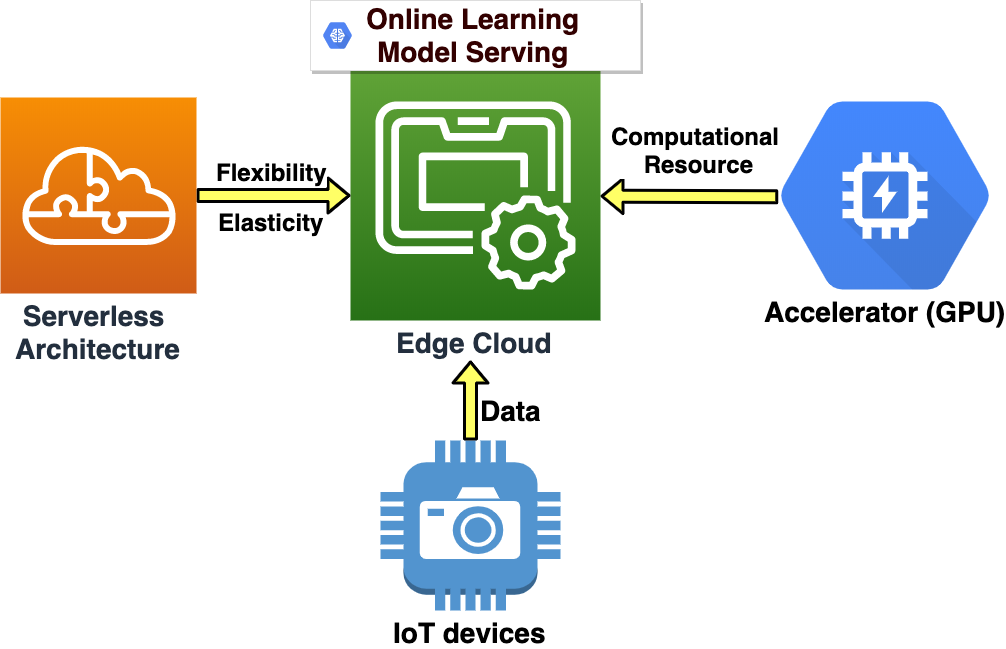
\includegraphics[scale=0.25]{figures/edge}
    \caption{The abstract design of STOIC -- a system for executing distributed machine learning applications in IoT (e.g. edge + cloud) settings.
\label{fig:edge}}
\end{figure}

Toward this end, we present STOIC -- a Serverless TeleOperable Hybrid Cloud. As depicted in Figure~\ref{fig:edge}, STOIC is a framework to which IoT devices stream data in batches for training and inference by machine learning applications.  The framework implements serverless computing and deployment for the applications. Unique to STOIC, however, is its scheduling system which intelligently places the application workload on edge and cloud systems that it predicts will result in the fastest time to completion. Moreover, STOIC takes advantage of GPU acceleration when available from the underlying cloud resource. In this paper, we discuss the design and implementation of this architecture, investigate the efficacy of using this extended serverless model for machine learning applications that span edge-cloud systems, and  empirically evaluate the performance of doing so. Using real workloads and deployments, we find that STOIC reduces the total response time of the applications we study from 6.48\% to 32.05\%, compared with four different runtimes, each running in isolation. In the system level evaluation, STOIC in duplicator mode successfully responds to 94.8\% of requested workloads with the least latency in a 24-hour experiment. Finally, we discuss related and future work and conclude.


%\section{Background}
%\label{sec:background}
%\input{background}

\section{STOIC}
\label{sec:STOIC}
\begin{figure}
    \centering
    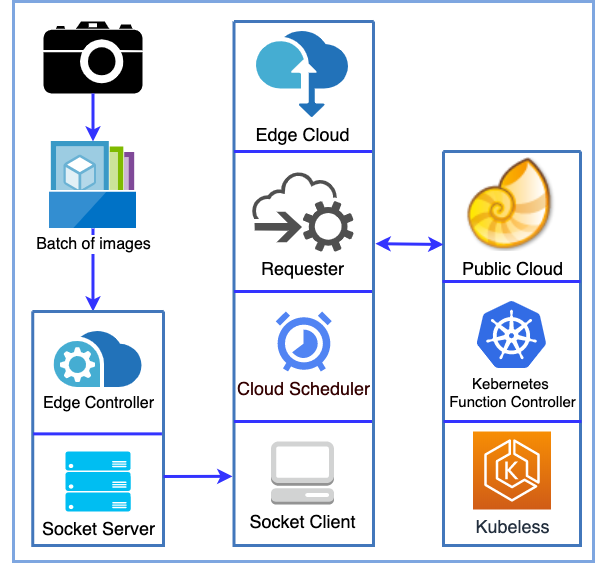
\includegraphics[scale=0.4]{STOIC}
    \caption{The STOIC Architecture \label{fig:STOIC}}
\end{figure}

To leverage hardware acceleration and distributed scheduling within a serverless architecture, we have developed STOIC, a framework for executing analytics applications in multi-tier IoT (sensing-edge-cloud) settings. STOIC streamlines the end-to-end process of packaging, transferring, scheduling, executing, and result retrieval for machine learning applications. Figure~\ref{fig:STOIC} shows three principal pillars of STOIC's architecture: Edge Controller, Edge Cloud, and Public Cloud.

\subsection{Edge Controller}
 We deploy a collection of edge devices, including multiple motion-detecting camera traps in open field and a local server as edge controller in the research facility at Sedgwick Natural Reserve~\cite{ref:sedgwick}. 
In this deployment, we install motion-triggered cameras (i.e. camera traps) at 
watering holes to capture images of wildlife in their natural habitat (as part of conservation science studies). The cameras are connected via a wireless radio to a computer located in an outbuilding at the reserve. We refer to this computer as the edge controller.  It is contectect to a private campus cloud via a microwave link. When a camera trap detects motion, it takes photos and persists the images in flash storage. Periodically, the camera traps transfer saved photos to the edge controller. STOIC runs on the edge controller and its execution is triggered by the arrival of batches of images from camera traps located across the reserve. When a batch arrives, STOIC partitions the image processing application (for object/animal classification) into tasks that it assigns to 1+ cloud components.
 
 \subsection{Edge Cloud}
 
As an intermediate computational tier between the sensors and public cloud, the edge cloud can be placed anywhere, preferably near the edge devices, to lower the response latency of analytics applications processing the images. Our edge cloud is currently deployed in our lab on campus which is connected to the edge controller via a fast network link.

Our edge cloud consists of a cluster of nine Intel NUCs~\cite{ref:nucs}.
Eucalyptus cloud system~\cite{ref:euca} manages the edge cloud and supports Linux virtual machine instances. Running on an instance, the STOIC socket client listens for the request from edge controller and then either executes the job locally on edge cloud or has STOIC requester interact with public cloud to complete the designated task.
 
 \subsection{Remote Public/Private Cloud}

To investigate the use of the serverless architecture with hardware accelerators, we employ a shared, multi-university, GPU cloud Nautilus~\cite{ref:nautilus} as our remote cloud system. Nautilus is an Internet-connected, HyperCluster research platform led by researchers at UC San Diego, National Science Foundation, the Department of Energy, and various participating universities globally.  Being designed for running data and computationally intensive applications, Nautilus uses Kubernetes~\cite{ref:k8s} as an interface to manage and scale containerized applications.  It uses Rook~\cite{ref:rook} to integrate Ceph~\cite{ref:ceph} data services. As of Nov. 2019, Nautilus consists of 141 computing nodes across the US and 422 GPUs are available in the cluster. All of these nodes are connected via a multi-campus network. In this study, we consider Nautilus as a public cloud that enables us to leverage hardware acceleration (GPUs) in the serverless architecture to serve edge devices. 
 
 \subsection{Implementation}
 
 Considering performance and interface, we
implement STOIC using Golang~\cite{ref:golang}. Golang provides high 
performance (vs scripting languages)and a user-friendly 
interface~\cite{ref:client-go} to Kubernetes.  STOIC currently supports
machine learning applications developed using the TensorFlow 
framework~\cite{ref:tensorflow}.
 
 \BlankLine
 \subsubsection{Serverless framework}
 For our serverless architecture, STOIC employs 
kubeless~\cite{ref:kubeless} and Docker~\cite{ref:docker} in the
 Nautilus Cloud. As a Kubernetes-native serverless framework, 
kubeless uses the Custom Resource Definition (CRD)\cite{ref:crd} to dynamically create functions as Kubernetes custom resources and launches runtimes on-demand. For specific machine learning tasks that STOIC executes, we use Docker to build customized runtime images that we upload to Docker 
Hub~\cite{ref:dockerhub} in advance. When the function controller 
at Nautilus Cloud receives a task request, it pulls the latest image 
from Docker Hub before launching the function. This deployment pipeline 
makes the runtime flexible and extensible for evolving applications. 
 
For the edge cloud, we execute tasks by directly invoking
the application function binaries. We make this design decision to simplify STOIC's control plane in  our prototype but we are investigating the use of
a consistent serverless architecture across edge and public/private 
cloud as part of future work.
 
 \BlankLine
 \subsubsection{STOIC Library Support}
 To leverage the computational power of the CPU systems available 
in the Edge and Public Cloud, we compile Tensorflow from source with AVX2, SSE4.2~\cite{ref:avx} and FMA~\cite{ref:fma} instruction set support. We then test the performance of customized Tensorflow package on three common machine learning training tasks: \textbf{(A)} \textit{Iris}~\cite{ref:iris} with 10-fold cross-validation; \textbf{(B)} \textit{MNIST}~\cite{ref:mnist} on 20 Epochs; \textbf{(C)} \textit{InceptionV3}~\cite{ref:v3} on 10 epochs with 1,000 images. 

We execute these applications 10 times on standard and customized Tensorflow packages. Table~\ref{tab:avx} shows the mean execution time of three benchmarks 
for each package. We calculate speed-up as $(T_s - T_c) / T_s$, where $T_s$ and $T_c$ represent the execution time by the standard and customized Tensorflow library respectively. We observe that, in all three benchmarks, the customized library achieves a speed-up that ranges from 17.4\% to 29.5\%. STOIC uses
the customized TensorFlow packages for cloud systems that implement these
instruction sets.  In our prototype, both the edge and public cloud have
these extensions.
 
 \BlankLine
 \subsubsection{GPU Accessibility}
 To enable GPU access by serverless functions, we build a container with NVIDIA Container Toolkit~\cite{ref:nvidia} support.  Such support includes the NVIDIA runtime library and utilities which link serverless functions to NVIDIA GPUs. We also install CUDA 10.0 and cuDNN 7.0 in the image.
 
\begin{table}
\centering
\scriptsize

\begin{tabular}{|c|c|c|c|} 
\hline
 & \textbf{Mean Std. (sec)} & \textbf{Mean Custom. (sec)} & \textbf{Speed-up \%}\\
\hline
\textbf{Iris} & 53.17 & 41.86 &  21.3\\
\hline
\textbf{MNIST} & 268.81 & 189.80 & 29.4 \\
\hline
\textbf{InceptionV3} & 958.47 & 791.28 & 17.4 \\
\hline
\end{tabular}

\caption{Performance comparison of Tensorflow library compiled with and without AVX2/SSE/FMA CPU instruction set support. The table shows the mean execution time across 10 runs and the corresponding speed-up percentage of three machine learning benchmarks.  \label{tab:avx}}
\end{table}
 
 \BlankLine
 \subsubsection{STOIC Runtime}
 To schedule the machine learning tasks across hybrid cloud deployments, we define four runtime scenarios: \textbf{(A)} \textit{edge} - A VM instance on the edge cloud with AVX2 support; \textbf{(B)} \textit{cpu} - A kubernetes pod on Nautilus containing a single CPU with AVX2 support; \textbf{(C)} \textit{gpu1} - A kubernetes pod on Nautilus containing a single GPU; \textbf{(D)} \textit{gpu2} - A kubernetes pod on Nautilus containing two GPUs. STOIC considers each of these deployment options as part of it scheduling decisions. Users can parameterize STOIC with their choice of deployment or allow STOIC to automatically schedule their applications.
 
 %For evaluation and canary deployment purpose, STOIC has implemented a feature flag of runtime that overrides the runtime selection made by scheduler when the user manually set the flag. This feature extensively helps evaluate the performance of STOIC, comparing with single-runtime schedulers.
 
 % STOIC executes tasks on the edge and cloud system for a warm up period (parameterizable but currently set to 1 hour) during which it observes deployment and execution times.
 
 \subsection{Execution Time Estimation}
 As depicted in Figure~\ref{fig:STOIC}, the STOIC socket server executes in the edge cloud and listens for requests from the edge controller (machine learning job requests). After a preset period (parameterizable but currently set to 1 hour), STOIC estimates total response time~($T_r$) of a requested batch, based on 4 different runtime scenarios. The total response time includes data transfer time~($T_t$), runtime deployment time~($T_d$) and corresponding processing time~($T_p$):
 
 \subsubsection{Transfer time~($T_t$)} measures the time spent in transmitting a compressed batch of images from edge controller to edge cloud and public cloud. We calculate transfer time as ${T_t = F_b / B_c}$ where $F_b$ represents the file size of batch and $B_c$ represents the bandwidth at the moment provided by a bandwidth monitor at edge controller. 
 
 \subsubsection{Runtime deployment time~($T_d$)} It measures the time Nautilus uses to deploy requested kubeless function. Since the scarcity of computation, it is common that \textit{gpu2} runtime takes longer to deploy than \textit{gpu1} and \textit{cpu} runtimes. We analyze the deployment log and calculate the average deployment time for each Nautilus runtime. In future work, we plan to develop a feedback control loop to dynamically update deployment time for each runtime. Note that, for \textit{edge} runtime, the transfer and runtime deployment time zero out since STOIC executes the task locally in the edge cloud.
 
 \subsubsection{Processing time~($T_p$)} is the execution time of a specific machine learning task. As a primary component for scheduling tasks across the hybrid cloud, we regress processing time based on prior experiment data by Bayesian Ridge Regression~\cite{ref:brr} due to its robustness to ill-posed problems compared to Ordinary Least Squares regression~\cite{ref:ols}. Thus, STOIC formulates the regression and uses it to predict the processing time based on the file size of the current batch. %Similarly to the runtime deployment time, we plan to construct a feedback control loop to dynamically update the coefficient and intercept of regression based on the incoming data of processing time as future work.
 
 \subsection{Workflow}
 The STOIC workflow is as follows: based on the three time components, STOIC predicts the total response times~($T_r$) of the four deployment options. The scheduler selects the runtime with the shortest estimated response time. Then the edge controller sends a request, including the payload of compressed image batch and runtime information, to edge cloud. Upon acceptance, the edge cloud executes the task locally if the choice is the \textit{edge} runtime. Such deployment is common when a batch of images is small. 

For large batch sizes, STOIC typically schedules one of the three public runtime options. For these three scenarios, the edge cloud first requests the deployment on public cloud. It then sends the payload to public cloud storage. The public cloud then deploys and executes the kubeless function. As a design decision, instead of running a requester pod in the public cloud, we run an instance on the edge cloud. We do so because the edge cloud is more stable and fault resilient than Nautilus which experiences intermittent downtime.  
 
Once Nautilus successfully deploys the serverless function, it informs the edge cloud's requester to trigger the function via an HTTP request. When the task completes, the requester retrieves the results and runtime metrics, and transmits them back to the edge controller. Finally, the controller saves the results and metrics to persistent storage. 
 
 \subsection{Intelligent Probing}
 With a series of experiments, we have found that the processing times from the same image batch and kubeless function can vary significantly between the first run and successive runs. This is due to the differences between cold and warm starts~\cite{ref:coldstart}.  A cold start is when a machine learning task requires retrieval of stored model and dataset from cloud storage, which takes time. Once the function retrieves and caches this information, sucessive invocations of the function (using the same container) avoid this cost (i.e. experience a warm start). 

STOIC accounts for cold and warm starts in its scheduling estimate using intelligent probes. When STOIC schedules the incoming task in a different runtime than the previous one, it triggers the function with the least amount of input data to ensure the function caches the model and dataset in memory. Following this, STOIC triggers the actual tasks. To avoid redundant probing, STOIC starts the task directly when the designated runtime is the same as the previous batch.


\section{Evaluation}
\label{sec:eval}
In this section, we empirically evaluate STOIC's performance when executing machine learning application. For every request, we run benchmark application on all available runtimes and compare the selection made by STOIC based on the predicted latency and the runtime with least total latency. In this section, we first describe the benchmark application that we consider, followed by our experimental setup and results. 

\subsection{Benchmark Application and Dataset}

We evaluate STOIC using an image processing application that classifies animal images from a wildlife monitoring system called ``Where's The Bear" (WTB)~\cite{ref:wtb}. ``Where's The Bear" is an end-to-end distributed data acquisition and analytics system that implements an IoT architecture and edge cloud. Our application makes inferences for each photo taken by deployed camera traps in Sedgwick Natural Reserve using a convolutional neural network (CNN)~\cite{ref:cnn}.  We train the model using labeled images from the WTB dataset. Technically, the application employs Tensorflow and Scikit-learn~\cite{ref:scikit} to implement image classification.  

In total, there are five classes that we consider in the CNN model training: Bird, Fox, Rodent, Human and Empty. Since class size is unbalanced due to frequencies of animal occurrences, we up-sample minority classes (e.g. fox) using the Keras ImageDataGenerator~\cite{ref:keras}.  Doing so ensures that the classification model is not biased. We resize every image in the WTB dataset to $1920 \times 1080$, and for each class, the dataset contains 251 images used to train the CNN model. Once model training is complete, the application stores this model in hdf5 format in cloud storage at both edge cloud (disk storage) and Nautilus (a shared volume in a Ceph file system).

To better harness the multiple GPU runtime in the public cloud, the application assigns each GPU to a spawned process, namely worker, and adds all images in the batch to a shared asynchronous queue. Upon the execution, all workers pick up the image job from the shared queue until it is exhausted. This mechanism ensures multiple GPUs evenly divide the workloads and achieve quasi-linear acceleration at application level, where the perfect linear speed-up is unattainable due to model loading and memory transfer overhead~\cite{ref:multi_gpu}. 

\subsection{Efficacy Experiments}

We first test the efficacy of STOIC by processing a sequence of image batches at four runtimes individually and then compare them with the determined runtime by STOIC. According to 2016 WTB dataset, the size of image batch fits to normal distribution $\mathbf{N}(\mu = 42.75, \sigma^2 = 39.5)$. To conduct an unbiased evaluation, we seed the simulator to make these image batches consistent across all runtimes and STOIC.


To make the result reliable, we conduct the experiment for a 24-hour time range, in which  154 image batches (616 executions) are processed by STOIC. Based on the data we observe, STOIC successfully selects the runtime of least latency by \textbf{85.1\%} of times (131 out of 154). We then compare the actual latency between the worst selection scenario and STOIC. The total latency of selected runtime by STOIC is 8041.06 seconds, whereas in the worst scenario the total latency is 18563.82 seconds. This indicates STOIC accelerates the execution of image processing by \textbf{2.3} times if the runtimes are erroneously selected by dispatcher.

\begin{figure}[t] \centering 
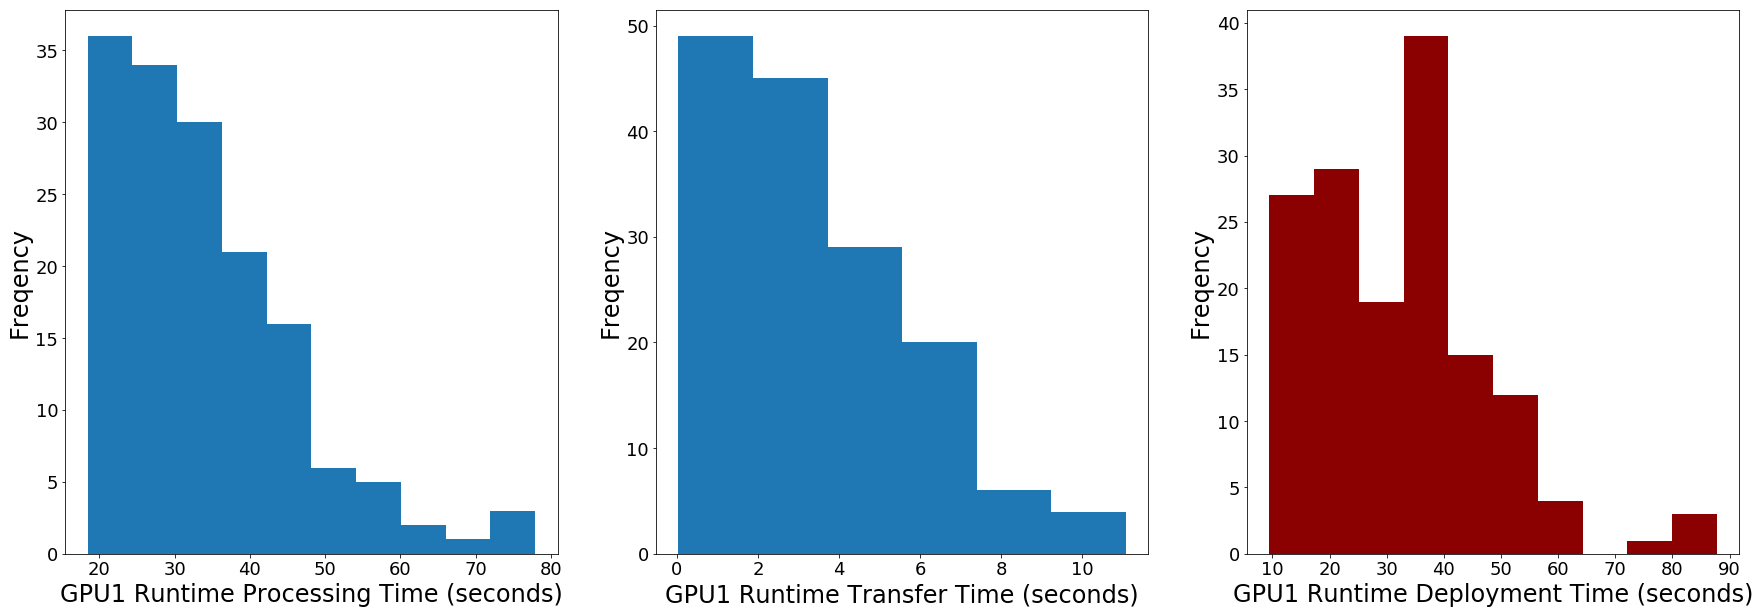
\includegraphics[scale=0.14]{gpu1_latency.png}
\caption{The distribution of three components in total response time~($T_r$): Processing time ($T_p$), Runtime deployment time ($T_d$) and Transfer time ($T_t$). The x-axis represents the time range, while the y-axis is the frequency of executions. The deployment time, which is depicted in the red histogram, is volatile and error-prone to prediction.
\label{fig:breakdown}}
\end{figure}

We further analyze the data points where STOIC made erroneous selection and found two sources of error. First, the most error occurs around two batch sizes where the total response time of runtimes have approximately same latency. To be specific, the edge and GPU runtimes cross over at 35 image batch size, and 90 image batch size for the GPU1 and GPU2 runtimes. At these cross-points, the close predictions of latency lead to incorrect selection. Second, the deployment time for GPU runtimes are volatile and error-prone to prediction. As a representative instance, Figure~\ref{fig:breakdown} demonstrates the distribution of processing time ($T_p$), transfer time ($T_t$) and deployment time ($T_d$) of GPU1 runtime. We observe geometric distribution from the histogram of processing time and transfer time, whereas deployment time varies irregularly with many outliers. These two phenomenons lead to mistaken selections in the experiment.

Further, we define an error metric, Mean Deadline Error (MDE), to better gauge the predictive capability of STOIC between edge cloud and GPU runtimes. Since the dedicated edge cloud is closer to the data source and more homogeneous and robust compared to public cloud, we are only concerned when GPU runtimes have longer total latency than edge cloud and STOIC deploys the workload to GPU runtimes. Mean Deadline Error is defined as $MDE = \frac{1}{n}\sum(L_g - L_e) \,|\ if \ L_g > L_e \ \& \ R_s = GPUx $, where $L_g$ is the latency of GPU runtime, $L_e$ is the latency of edge cloud, $R_s$ is the selected runtime by STOIC. Based on the experiment data, the MDE gpu1 is \textbf{26.68} seconds (44.18\% to the mean gpu1 runtime latency) and MDE gpu2 is \textbf{43.98} seconds (47.43\% to the mean gpu2 runtime latency). This result implies that the unstable deployment time of GPU runtimes significantly affects the accuracy of prediction made by STOIC. 

\begin{figure}[t] \centering 
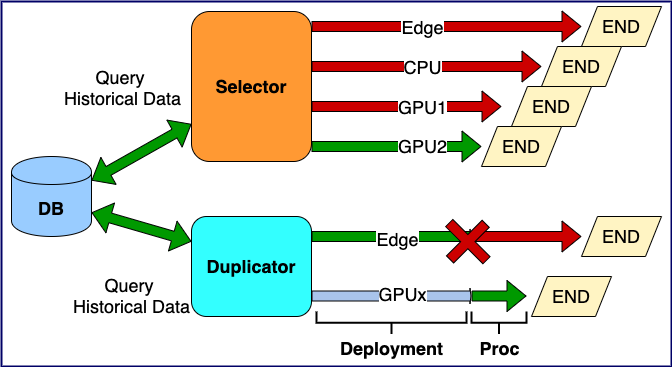
\includegraphics[scale=0.35]{selector_duplicator.png}
\caption{The selector and duplicator modes of STOIC. 
\label{fig:duplicator}}
\end{figure}

To address the above issue, we reconfigure STOIC into the duplicator mode demonstrated in Figure~\ref{fig:duplicator}. Based on the historical data, the selector makes prediction and only execute workload at the runtime with least total latency, whereas the duplicator runs workload on edge cloud and GPU runtimes concurrently, and halts the edge cloud execution if the remaining time at edge cloud is longer than the expected processing time ($T_p$) at the GPU runtime once it completes deployment. Under this mode, STOIC is able to make right selection between edge cloud and GPU1 runtime and promptly respond to the request \textbf{96.7\%} of times (149 out of 154). 

In the case of gpu2 runtime, it has more variable deployment and processing time compared to gpu1 runtime, which possibly leads to lower success rate of selection. The analytics of the data proves this assumption that STOIC makes right selection between edge cloud and gpu2 runtime by \textbf{94.8\%} (146 out of 154) of times, 1.9\% lower than being with gpu1 runtime. However, the total latency of gpu1 runtime (154 image batches) is \textbf{8872.65} seconds, whereas the total latency is \textbf{8396.9} seconds for gpu2 runtime. We argue that even though STOIC make more mistakes for gpu2 than gpu1, the duplicator mode of edge cloud versus gpu2 makes the entire end-to-end system faster and more efficient. We plan to investigate runtimes with more GPUs and the trade-off between the predictability and efficiency of system as future work.


\section{Related Work}
\label{sec:relate_work}
As related work, we consider recent advances in both machine learning infrastructure and serverless computing domains. In the former area, much research has extended efforts into designing efficient systems for inference and deployment of machine learning models. As a complement to the Tensorflow framework, Tensorflow-serving~\cite{ref:tensorflow-serving} integrates new models and updates versions from training to serving. Though it makes seminal exploration on the multi-tenant model hosting service, Tensorflow-serving does not realize authentic high-performing parallelism to handle concurrent heavy query loads. 

Clipper~\cite{ref:clipper} constructs a general-purpose low-latency prediction serving system, which attempts to solve the problem of demanding real-time prediction at the client-side and handling heavy query load at the server-side. It also enables the model composition and online learning to improve accuracy and render more reliable predictions. To explore the multi-pipeline techniques, PRETZEL~\cite{ref:pretzel} casts model-serving as a database problem and applies multi-query optimizations to maximize performance. However, both Clipper and PRETZEL require considerable compute resources in caching, batching, adaptive model selection and off-line training to maximize throughput. Therefore, they are not optimized for resource constrained and heterogeneous, multi-tier IoT systems. 
To the best of our knowledge, STOIC is the first work to addresses this problem by integrating machine learning applications into a serverless architecture that leverages GPU as additional computational resources for IoT devices. We consider it as a promising and extensible solution for high-throughput and low-latency system for online training and machine learning applications in general. 

 To build an end-to-end system for practical machine learning applications, we require several other components. Seneca~\cite{ref:seneca} fine-tunes hyper-parameters of machine learning models on a general-purpose serverless architecture (AWS Lambda~\cite{ref:lambda}). It provides a fast and low-cost method to grid search for the best-performing hyper-parameter set, which is essential in the deployment pipeline of machine learning applications. Velox~\cite{ref:velox} offers a low-latency and scalable solution for complex analytical model-serving, in which it completes a missing piece of personalized prediction serving using Apache Spark~\cite{ref:spark}. For calibrating performance, McGrath et al.~\cite{ref:serverless} propose an empirical methodology to measure the design and performance of serverless platforms, including latency and auto-scaling capability. These related systems are complementary to STOIC and can be combined together
to provide a robust serverless ecosystem for machine learning applications.



\section{Conclusion}
\label{sec:conclusion}
In this paper, we propose a framework, called STOIC, for executing machine learning applications in hybrid cloud settings based on serverless architecture. STOIC integrates three components: Edge Controller, Edge Cloud, and Public Cloud. When the scheduler at edge controller receives a batch of images from open field camera traps, it predicts the total response time for processing the batch based on batch size and historical log data. It then schedules the task to the runtime that it predicts to have the least total response time.  Our STOIC prototype considers four different runtime scenarios. When STOIC schedules the task to the public cloud, the edge cloud deploys a serverless function and then relays the request and payload to the public cloud. STOIC returns the result and metrics back to edge controller when the task completes.

We present the design principles, implementation details, workflow and empirical evaluation on real-world machine learning application for STOIC. Our evaluation demonstrates STOIC is able to intelligently schedule machine learning tasks across hybrid cloud deployments and obtain better performance that using any single deployment option in isolation.  Our speed-up percentages range from 6.48\% to 32.05\% for the application and datasets that we study.

As part of future work, we are developing a feedback control loop to dynamically update the deployment and processing time of STOIC tasks. We plan to also investigate the feasibility of executing model-training tasks using STOIC. Finally, we plan to investigate ways of not having sufficient labeling for image classification tasks and to unify the serverless architecture across all edge and cloud systems within the STOIC system and for the applications that execute using it.



\section*{Acknowledgments}
This work has been supported in part by NSF (CNS-1703560, CCF-1539586,
ACI-1541215), ONR NEEC (N00174-16-C-0020),
and the AWS Cloud Credits for Research program.


% references section
\bibliographystyle{IEEEtran}
\bibliography{ref}
% \end{thebibliography}

\end{document}
